%%%%%%%%%%%%%%%%%%%%%%%%%%%%%%%%%%%%%%%%%%%%%%%%%%%%%%%%%%%%%%%%%%%%%%%%%%%%%%%%%%%%%%%%%%%%%%%%%%%%%%%%%%%%
%%%%%%%%%%%%%%%%%%%%%%%%%%%%%%%%%% DATA   %%%%%%%%%%%%%%%%%%%%%%%%%%%%%%%%%%%%%%%%%%%%%%%%%%%%%%%%%%%%%%%%%
%%%%%%%%%%%%%%%%%%%%%%%%%%%%%%%%%%%%%%%%%%%%%%%%%%%%%%%%%%%%%%%%%%%%%%%%%%%%%%%%%%%%%%%%%%%%%%%%%%%%%%%%%%%%

\section{Data and Descriptive Statistics} \label{sec:dataoob}

\subsection{Data sources and sample} 
We use administrative data from the Austrian Social Security Database (ASSD), which covers all social insurance episodes and provides information on demographics, employment sectors, labor income, and spells of employment and unemployment. We augment the ASSD with variables from the Federal Ministry of Labor and Economy (BMAW), including protection type, asylum date, participation in educational programs, language proficiency, marital status, residency ZIP codes, basic income support, education level, previous and desired professions. This supplementary data covers all individuals granted protection status and registered with the Austrian Public Employment Service (PES) at any point in time. Although registration at the PES is voluntary, access to the social benefits linked to registration encourages it. In Appendix~\ref{subsec:pes_selection}, we test whether the number of refugees in our data, as a share of all individuals from those countries of origin in a district, correlates with our main explanatory variables, which is not the case.  %Still, we address potential sample selection biases in Section~\ref{identification}.

Asylum-seekers are granted special health insurance upon arrival, designated as ``O4'' or ``OE'' in the ASSD, signaling coverage under basic subsistence support. This unique classification enables the precise identification of asylum-seekers, distinguishing them from recipients of other insurance types. It also allows us to see whether subsidiary-protected individuals still receive this form of welfare benefits after being granted protection.

Our analysis encompasses all refugees granted protection under the Geneva Convention or subsidiary protection between January 2011 and August 2018.\footnote{The selection of 2011 as the starting point is due to improved data quality from this year onwards. The cutoff in August 2018 allows for a five-year observation period following the granting of protection status.} We focus on individuals aged 18 to 60 at the time of immigration, excluding those who were granted protection status on the day of arrival, indicative of family reunification. We further exclude refugees for whom calculating treatment variables was impractical,\footnote{In a few districts, the $IVUR$ could not be computed for certain observations during the early years of our observation period due to official zeroes in the unemployment count.} and individuals receiving protection more than three years after arrival.\footnote{We conduct robustness exercises with different sample restrictions in Section~\ref{subsec:robustnessoob}.}

Our final sample consists of 41,212 refugees, among whom 39,694 maintained active insurance coverage for a minimum of five years post-protection. In Section~\ref{no_insurance} of the Appendix, we examine the impact of our treatment variables on the probability of continuous insurance coverage over this five-year span. Finding no significant influence, we consequently limit our further analysis exclusively to those individuals who can be observed until the end of the five-year period.

Additionally, we enhance our dataset with detailed municipality characteristics from Statistics Austria and utilize the ASSD to ascertain the number of vacancies and unemployed individuals at the district level.


\subsection{Treatment variables}

\vspace{0.3cm}
\textbf{Initial vacancy-to-unemployment ratio \textit{(IVUR).}} \hspace{0.5cm} We characterize labor market tightness at the time of protection status receipt through the initial vacancy-to-unemployment ratio ($IVUR$), utilizing aggregated monthly data on registered unemployment and vacancies at the municipality level from the ASSD. The $IVUR$ is defined as follows:

\begin{equation}
\label{eq:IVUR}
IVUR_{d_0,t_0} = \frac{\sum_{t=0}^{2} \text{open positions}_{d_0, t}}{\sum_{t=0}^{2}\text{unemployed individuals}_{d_0, t}}
\end{equation}

This ratio is calculated by dividing the sum of open positions by the sum of unemployed individuals within a regional entity during the first three months following protection status receipt. $t_0$ refers to the month of receiving protection. $d_0$ refers to the district of residence when receiving protection. We choose political districts as they roughly align with labor markets.%\footnote{In Appendix XX, we investigate alternative regional aggregations and find that results are highly robust. (TO BE INCLUDED)}


\vspace{0.5cm}
\noindent\textbf{Initial Potential Benefit Level \textit{(IPBL).}} \hspace{0.5cm} Using the information on benefit levels introduced in Section~\ref{sec:background}, we define the Initial Potential Benefit Level ($IPBL$) as follows:

\begin{equation}
\label{eq:IPBL}
IPBL_{f,p,s_0,t_0} = \frac{PB_{f,p,s_0,t_0}}{1000}
\end{equation}

The $IPBL$ measures the monthly benefits available to a refugee with no other income or wealth. It depends on family status $f$,\footnote{We determine family benefit eligibility if a person's child is insured in Austria or if there is a partnership status with another asylum-seeker and at least one dependent child co-insured in Austria at the time of protection receipt. This is different from our family arrival variable used to define the arrival groups in our identification strategy, where we consider asylum-seekers who arrive in Austria on the same date.} type of protection $p$, state of residence at the time of protection $s_0$, and the date of protection $t_0$. We present $IPBL$ in units of 1,000 euro to facilitate a clearer graphical presentation of our findings. Consequently, $IPBL$ varies across federal states, protection statuses, family statuses, and over time, reflecting a sequence of policy reforms. A caveat is that our measure of benefit eligibility is imperfect, not covering other forms of benefits and only approximating the benefits for families. However, variation induced by the reforms should be captured very well. A second caveat is that $IPBL$ measures \emph{potential} rather than \emph{received} benefits. Refugees in private accommodation are directly affected by the cash component captured by $IPBL$, while refugees in organized accommodation receive most support in-kind and are only indirectly exposed---through the changed value of moving to private accommodation. As we do not observe accommodation type at the individual level, the $IPBL$ coefficients in Section~\ref{sec:results} average over both groups. We return to the implications for interpretation in Section~\ref{sec:discussion}.

Importantly, both $IVUR$ and $IPBL$ are assigned to each individual upon the granting of protection and remain unchanged thereafter. These indicators reflect the labor market tightness and the welfare benefits system that an asylum-seeker is subject to at the moment of initial authorization to enter the labor market and to move within Austria. Later changes in these variables due to relocation, amendments to benefit rules, or economic conditions are not considered as they are no longer assigned exogenously.

\subsection{Outcomes}

We examine three categories of outcomes at the individual level: labor market integration, mobility, and social support. %, utilizing administrative records from the social security agency and the PES. 
We express each metric on a monthly basis, with time standardized relative to the month of protection receipt. Labor market performance encompasses a) an indicator for being employed\footnote{Employment is defined as any employment spell subject to social insurance contributions.}, b) being in marginal employment\footnote{Marginal employments are employment spells with earnings below the marginal earnings threshold (€406 in 2015).}, c) monthly real labor earnings, and d) logged real monthly wage income\footnote{The earnings used to calculate real labor earnings and logged real monthly wage income are reported as pre-insurance, pre-tax gross income for each employer-employee relationship. For employment spells before 2019, earnings were reported annually, while after 2019, they have been reported on a monthly basis. We calculated average daily earnings for each employment contract and summed them up in cases of multiple simultaneous spells.}. For mobility, we track whether a refugee remains in the same state as when protection was granted and whether they reside in Vienna, specifically for those initially located in a different federal state. The mobility measure is based on the contact address available to the Social Security Administration. 
Social support metrics include a) receipt of any Public Employment Service (PES) support within a month, such as language courses, job training, or counseling, and b) receipt of any welfare benefits, and separated by basic needs support and basic subsistence support sources. Additionally, an active insurance spell serves as a proxy for a refugee's presence in Austria.\footnote{Our focus on individuals who received protection makes it rather unlikely that individuals switch to an informal status and remain in Austria, which would be an alternative explanation for an end to insurance in Austria.}

\FloatBarrier


\subsection{Descriptives}

Table~\ref{tab:summarystatistics} presents the summary statistics for our analysis sample, which consists of 39,694 individuals. Among these, 31,597 are Convention refugees, and 8,097 have subsidiary protection status. Two-thirds of refugees (64.7\%) are male, with an average age of 30.49 years at the time of immigration. More than half of the sample, 54.6\%, originates from Syria, followed by significant populations from Afghanistan (18.5\%), Iraq (7.8\%), and Iran (7.3\%). A substantial portion, 59.6\%, exhibits limited German language proficiency (A1/A2 level), and 69.2\% possess only primary education or lack it entirely. Noteworthy disparities exist between Convention refugees and subsidiary-protected individuals regarding their countries of origin, the duration of asylum processes (12.1 months for Convention refugees versus 15.9 months for those with subsidiary protection), and their eligibility for family benefits\footnote{We define eligibility for family benefits when receiving protection for refugees as applicable to those who are co-insured or provide co-insurance--- through a partnership or a parent-child relationship---to another individual who has been registered as a refugee in Austria on or before the date of protection.} (35.9\% versus 24\%). $IVUR$ is similar across groups, but on average, the $IPBL$ for subsidiary-protected individuals is €308 lower due to a lower likelihood of being eligible for family benefits and generally less generous benefits for this group (see Section~\ref{sec:background}).

The final panel of the table details outcomes measured in the 12\textsuperscript{th} month post-protection. Around 95\% have an active insurance spell. The employment rate is 11.3\% with mean monthly earnings of €203. Subsidiary-protected refugees do slightly better than Convention refugees on both metrics. 71\% of Convention and 61\% of subsidiary-protected refugees still live in the same state as initially assigned to. Given the low labor market integration, dependence on welfare benefits is high; 75\% receive some form of benefits, and approximately 38\% receive support from the PES.

\begin{table}
    \caption{Summary statistics}
    \label{tab:summarystatistics}
    \begin{threeparttable}
        \begin{small}
          %  \resizebox{\linewidth}{!}{%
                \begin{tabular}{lcccc}
                    %\expandableinput
                    \begin{tabular}{lccc}
\toprule
 & Convention refugee & Subsidiary-protected & Total \\
\midrule
\multicolumn{1}{l}{} & \multicolumn{3}{c}{Time-invariant characteristics} \\
Gender (female=0) & 0.63 (0.48) & 0.70 (0.46) & 0.65 (0.48) \\
Age at immigration & 30.75 (9.17) & 29.49 (9.46) & 30.49 (9.25) \\
Origin country & & & \\
\quad Afghanistan & 4440 (14.1\%) & 2903 (35.9\%) & 7343 (18.5\%) \\
\quad Iran & 2779 (8.8\%) & 124 (1.5\%) & 2903 (7.3\%) \\
\quad Iraq & 1806 (5.7\%) & 1287 (15.9\%) & 3093 (7.8\%) \\
\quad Other & 1623 (5.1\%) & 639 (7.9\%) & 2262 (5.7\%) \\
\quad Russia & 433 (1.4\%) & 158 (2.0\%) & 591 (1.5\%) \\
\quad Somalia & 631 (2.0\%) & 1190 (14.7\%) & 1821 (4.6\%) \\
\quad Syria & 19885 (62.9\%) & 1796 (22.2\%) & 21681 (54.6\%) \\
Duration asylum process & 12.08 (9.02) & 15.90 (9.50) & 12.86 (9.25) \\
German skill level & & & \\
\quad A & 18786 (59.5\%) & 4872 (60.2\%) & 23658 (59.6\%) \\
\quad B/C & 6019 (19.0\%) & 1258 (15.5\%) & 7277 (18.3\%) \\
\quad unknown & 6792 (21.5\%) & 1967 (24.3\%) & 8759 (22.1\%) \\
Education level & & & \\
\quad primary & 21344 (67.6\%) & 6122 (75.6\%) & 27466 (69.2\%) \\
\quad secondary & 4469 (14.1\%) & 640 (7.9\%) & 5109 (12.9\%) \\
\quad tertiary & 1913 (6.1\%) & 219 (2.7\%) & 2132 (5.4\%) \\
\quad unknown & 3871 (12.3\%) & 1116 (13.8\%) & 4987 (12.6\%) \\
Family benefit eligibility & 0.36 (0.48) & 0.24 (0.43) & 0.34 (0.47) \\
\multicolumn{1}{l}{} & \multicolumn{3}{c}{Initial local conditions} \\
IVUR & 0.19 (0.15) & 0.20 (0.16) & 0.19 (0.15) \\
IPBL (in €1,000) & 0.83 (0.29) & 0.52 (0.29) & 0.76 (0.32) \\
\multicolumn{1}{l}{} & \multicolumn{3}{c}{Outcomes in month twelve} \\
No Austrian insurance & 0.06 (0.23) & 0.03 (0.16) & 0.05 (0.22) \\
In employment & 0.10 (0.30) & 0.17 (0.37) & 0.11 (0.32) \\
Monthly real earnings & 180.27 (551.53) & 292.51 (663.54) & 203.16 (577.92) \\
In marginal employment & 0.03 (0.18) & 0.03 (0.18) & 0.03 (0.18) \\
Residency in initial state & 0.71 (0.45) & 0.61 (0.49) & 0.69 (0.46) \\
Residency in Vienna & 0.51 (0.50) & 0.58 (0.49) & 0.52 (0.50) \\
PES services & 0.38 (0.48) & 0.39 (0.49) & 0.38 (0.49) \\
Receiving welfare benefits & 0.76 (0.43) & 0.74 (0.44) & 0.75 (0.43) \\
\midrule
Observations & N=31597 & N=8097 & N=39694 \\
\bottomrule
\end{tabular}
                \end{tabular}
        %    }
        \end{small}
       % \vspace{-1em}
        \begin{tablenotes}
           % \parbox[t]{\textwidth}{%  % Set a strict width to the text width
           \footnotesize
                \item {\textit{Notes:} The table reports means and standard deviations (in brackets) for continuous and binary variables. The number of observations and the percentage within groups are reported for categorical variables. Time-varying (outcome) variables are reported for the 12\textsuperscript{th} month after protection was received. The sample is restricted to refugees who received protection between January 2011 and August 2018, who were between 18 and 60 years old at the time of immigration and whose asylum process lasted longer than a day but less than three years, and where full data is available for 60 months after the date of protection. Family benefit eligibility is an indicator equal to one if children who are co-insured with this person or their partner are registered in Austria at the time of receiving protection. Duration of asylum process is denoted in months, earnings are denoted in real 2015 euros, and IPBL is denominated in €1,000 (real 2015 values) to match the convention used throughout the regression analysis and all figures.}
   %         }
        \end{tablenotes}
    \end{threeparttable}
\end{table}

Figure~\ref{fig:descriptive_outcomes_main} shows how the employment rate (left) and the share of refugees who remain in the initial state (right) evolve from the moment of receiving protection. The employment rate starts from near zero at the time of protection. For men, it rises steadily and reaches about 60\% after five years. For women, the employment rate is less than 20\% after five years. The other notable aspect is high mobility rates immediately after receiving protection. Within six months, a quarter of refugees have moved to another state. Mobility is higher for men than for women. Figure~\ref{fig:descriptive_outcomes_appendix} in the Appendix shows the evolution of other outcome variables by gender over time.



\begin{figure} 
    \caption{Share of refugees in employment and residency in initial state by time since receiving protection} %\\ by months since protection was received.}
    \label{fig:descriptive_outcomes_main}
    \begin{center}        
        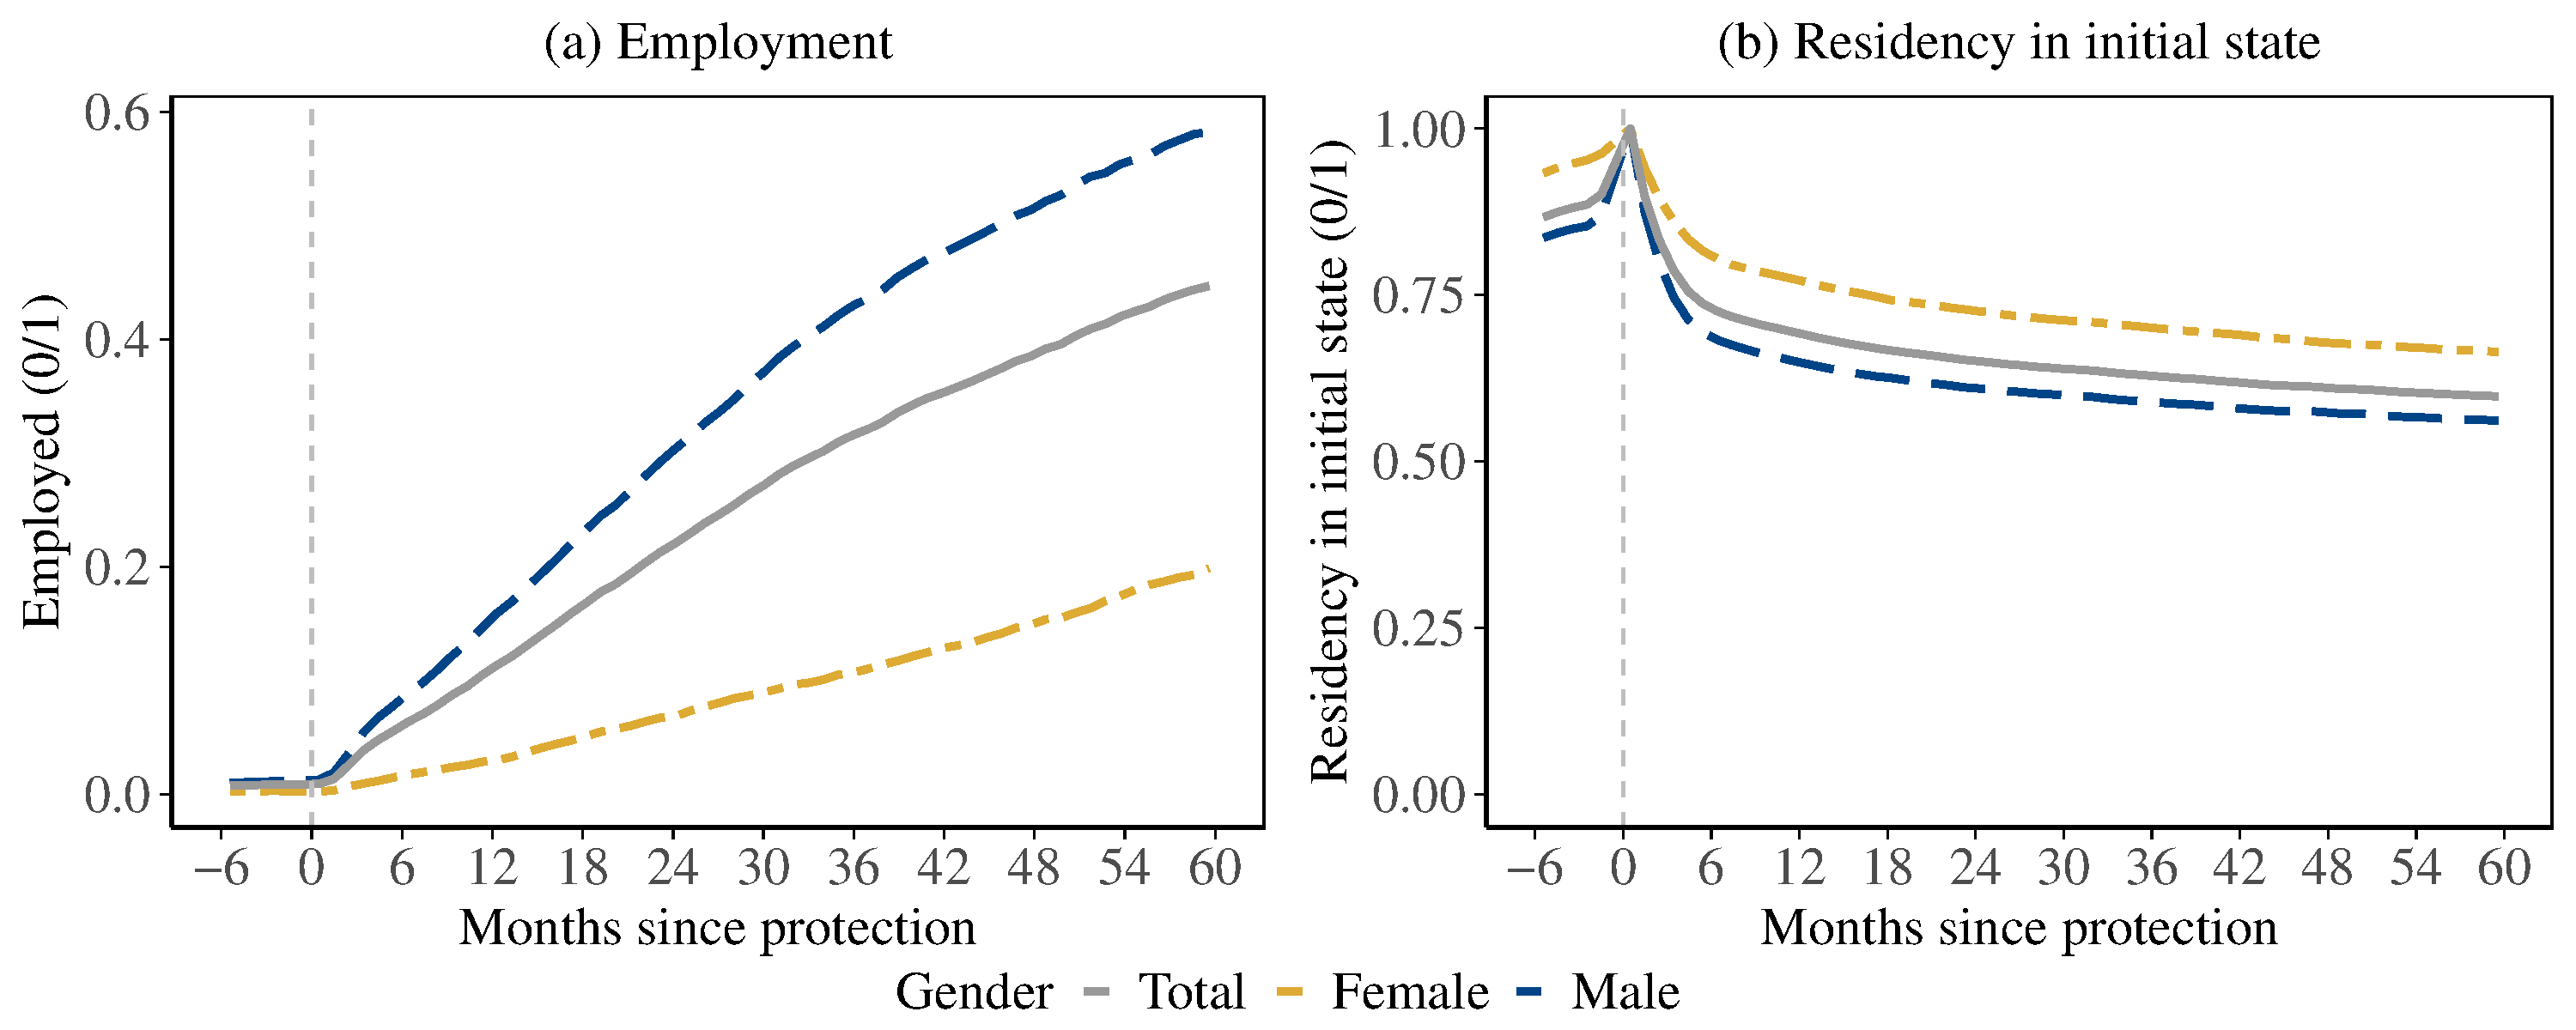
\includegraphics[scale=0.3]{figures/fig_descriptive_outcomes_main.pdf}
    \end{center}
% \\
       \justify 
 	{\footnotesize 
 		\textit{Notes:}   
%\fignote{Notes: 
The figure shows the share of employed refugees and of refugees who remained in their initial state by months since protection and gender. The x-axis shows the months since receiving protection. The y-axis displays the shares of refugees in (a) employment or (b) residing in the state of protection (initial state).}
\end{figure}

Mobility patterns after receiving protection vary substantially between federal states (see Figure~\ref{fig:movermatrix}). In Vienna, 96\% of refugees remain, while only 26\% do so in Burgenland, the other end of the distribution. The overwhelming majority of individuals who move between federal states move to Vienna. Twelve months after protection, 90 or more percent of all refugees are either in their initial states or in Vienna. The other states play only a marginal role as destinations for internal mobility.

\begin{figure} 
    \caption{Residence of refugees twelve months after receiving protection by initial state} %\\ by months since protection was received.}
    \label{fig:movermatrix}
    \begin{center}               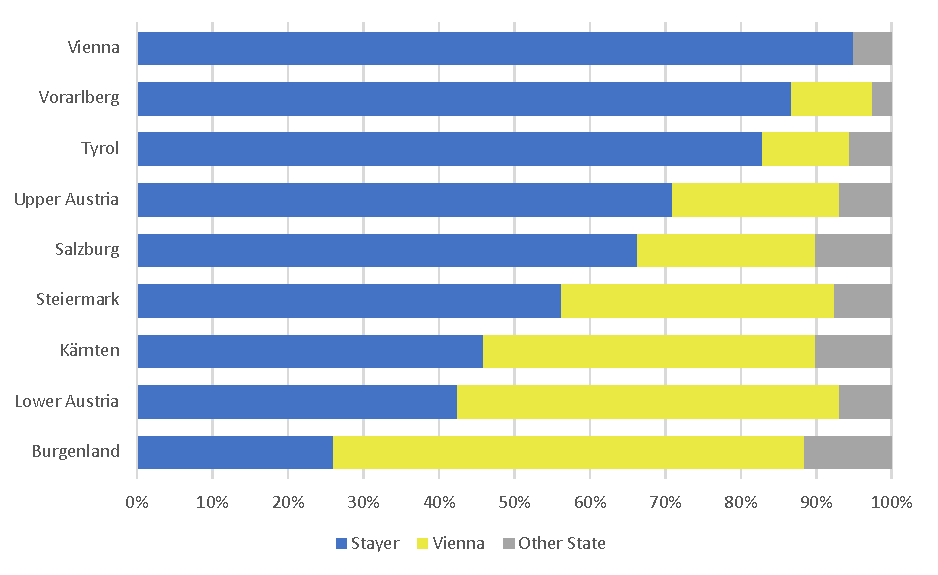
\includegraphics[width=0.7\textwidth]{figures/fig_movermatrix.pdf}
    \end{center}
%\fignote{Notes: 
  \justify 
 	{\footnotesize 
 		\textit{Notes:} The figure shows the state of residence of refugees twelve months after receiving protection. Stayers remain in the initial state (blue). Yellow bars indicate the shares that move from another state to Vienna. Gray bars indicate the shares that move to a state other than Vienna. %XXX: CLARIFY WHETHER THIS IS THE SAME SAMPLE AS IN PREVIOUS FIGURE
}
\end{figure}

Vienna is not only an attractive destination among refugees but also among other migrants. While 22\% of the Austrian population live in Vienna, this share is about 40\% among foreigners. On the other end, Burgenland, with 3.3\% of the population, only hosts 2\% of foreigners in Austria \citep{statistikaustria_2024}.
% \begin{figure}[htbp]
%     \centering
%      \caption{Evolution of positive decisions from BMI and our proxy for family reunified members, 2016-2022, quarterly}
%     \includegraphics[width=0.8\textwidth]{bmi_assd6m_en.png}
%        \label{fig:bmiassd}
% \end{figure}

